% Copyright (c) 2009-2014 Ilya Palachev <iliyapalachev@gmail.com>

% Declare the class of document: size of paper, size of font, and etc.
% Type of the document is "article".
\documentclass[a4paper, 12pt, titlepage]{article} 

% Package that enables setting the size of free spaces at the border of the 
% page with the command  \geometry :
\usepackage{geometry}
\geometry {
   left=3cm,
   right=1.5cm,
   top=2cm,
   bottom=2cm
}

\usepackage[utf8]{inputenc}

\usepackage[english,russian]{babel}

\usepackage{amsmath}

%\usepackage{cmap}

\usepackage{indentfirst}

\usepackage{a4wide,amssymb}

%\usepackage[pdftex]{graphicx}

%\usepackage{wrapfig}

%\linespread{1.3}               % полтора интервала. Если 1.6, то два интервала
\pagestyle{plain}               % номерует страницы

\usepackage{graphicx}
\renewcommand{\topfraction}{1}
\renewcommand{\textfraction}{0}

% Package that enables usage of theorems and definition designed in a 
% standard way.
% http://en.wikibooks.org/wiki/LaTeX/Theorems
\usepackage{amsthm}

% Create environment for smart definitions
\theoremstyle{definition}
\newtheorem{SmartDefinition}{Определение}

% Create environment for smart theorems
\theoremstyle{plain}
\newtheorem{SmartTheorem}{Теорема}

% Create environment for smart lemmas
\theoremstyle{plain}
\newtheorem{SmartLemma}{Лемма}

% The following code enables back references:
\usepackage{color} 
\definecolor{darkgreen}{rgb}{0,.5,0} 
\usepackage[unicode,colorlinks,filecolor=blue,citecolor=darkgreen,pagebackref]
{hyperref}

% The package that provides symbols like \Square:
\usepackage{wasysym}

%opening
\title{Опорные методы восстановления выпуклых тел и их обобщения для задачи
восстановления многогранников по теневым и бликовым контурам \\ Технический
отчет}
\author{Палачев Илья}

\begin{document}

\maketitle

\tableofcontents

%%%%%%%%%%%%%%%%%%%%%%%%%%%%%%%%%%%%%%%%%%%%%%%%%%%%%%%%%%%%%%%%%%%%%%%%%%%%%%%%

\section{Введение}

\subsection{Исходная практическая проблема восстановления моделей алмазов по
теневым и бликовым контурам}

\subsection{Описание технологии построения моделей алмазов}

\subsection{Погрешности в теневых контурах и их последствия}

\subsection{Можно ли корректировать теневые контуры?}

\subsection{Смежные проблемы в компьютерной томографии, магнитно-резонансной
визуализации и обработке данных лазерного радара}

\subsection{Обзор работы}

%%%%%%%%%%%%%%%%%%%%%%%%%%%%%%%%%%%%%%%%%%%%%%%%%%%%%%%%%%%%%%%%%%%%%%%%%%%%%%%%

\section{Основные понятия: преобразование двойственности и опорное представление
выпуклого тела}

Ключевыми понятиями, использующимися в данной работе для решения задачи
восстановления трехмерных тел являются понятие \textbf{преобразования
двойственности} и понятие \textbf{опорной функции выпуклого тела}. Первое из
них активно используется для решения задач вычислительной геометрии, поскольку
оно позволяет путем несложных преобразований над входными данными
переформулировать задачу так, чтобы понятия "точка" и "плоскость" поменялись
местами, что позволяет сводить новые задачи к таким, для которых уже имеются
известные методы решения. Примерами приложений преобразования двойственности
являются такие задачи как:

\begin{itemize}
 \item Нахождение пересечения многогранников.
 \item Нахождение треугольника минимальной площади с вершинами на заданном
множестве точек \cite{journals/BIT/ChazelleG1985}
 \item Разбиение множества точек на плоскости прямой на 2 класса, лежащих по
 разные стороны от прямой
\end{itemize}

и многие другие.

Второе понятие широко используется в такой области как \textbf{геометрическая
томография}. Суть подхода состоит в том, что любое выпуклое тело однозначно
определяется своей опорной функцией и задачу восстановления тела можно свести к
задаче восстановления опорной функции этого тела. В работе
\cite{journals/cviu/GhoshK98} производится анализ опорного представления и,
между прочим, исследуется его связь с преобразованием двойственности.

\subsection{Понятие полярного преобразования двойственности}

Термин преобразования двойственности имеет хождение в вычислительной геометрии,
где он нашел широкое применение. В проективной геометрии данное понятие имеет
сходство с понятием поляры.

\begin{SmartDefinition}
 Пусть $\mathbb{R}^{n}$ - евклидово пространство. \textbf{Преобразованием 
двойственности} называется отображение $\delta$, определенное на множествах
аффинных подпространств пространства $R^{n}$, не содержащих начало координат
$0 = (0, \ldots, 0)$, и действующее следующим образом:
\begin{itemize}
 \item Пусть $A \neq 0$ -- подпространство размерности $0$ (т. е. точка),
 $A = (a_{1}, a_{2}, \ldots, a_{n}) \neq 0$. Тогда ему ставится в
 соответствие аффинное гиперпространство $\delta(A)$, описываемое линейным
 уравнением $a_{1} x_{1} + a_{2} x_{2} + \ldots + a_{n} x_{n} = 1$.
 \item Пусть $L$ -- некоторое аффиное гиперпространство (т. е. 
 подпространство размерности $n - 1$), не содержащее начало координат. Тогда его
 можно описать с помощью уравнения
 $a_{1} x_{1} + a_{2} x_{2} + \ldots + a_{n} x_{n} = 1$, причем коэффициенты
 этого уравнения определяются однозначно. Тогда преобразование двойственности
 ставит в соответствие $L$ точку $\delta(L) = (a_{1}, a_{2}, \ldots, a_{n})$.
 \item Пусть $L$ -- подпространство размерности $k \neq 0, n - 1, n$. Тогда ему
 ставится в соответствие подпространство размерности $n - k - 1$, определяемое
 как $\delta(L) = \{\delta(M) \; | \; L \subset M, dim M = n - 1\}$.
\end{itemize}

\end{SmartDefinition}

%% TODO: Добавить утверждение о том, что преобразование двойственности сохраняет
%% инцидентность

\subsection{Пересечение многогранников и построение выпуклой оболочки --
двойственные задачи}

Свое распространение в вычислительной геометрии преобразование двойственности
получило благодаря статье Мюллера - Препараты \ref{Muller1978217}, в которой
описывается метод построения пересечения выпуклых многогранников. Он описан
также в классической монографии Препараты - Шеймоса "Введение в вычислительную
геометрию" \ref{Preparata:1985:CGI:4333}. Основная идея заключается в том, что
преобразование можно расширить на класс многогранных тел, если сопоставлять
вершинам -- грани, граням -- вершины, а всякому ребру, соединяющему некоторые
две точки $A_{1}$ и $A_{2}$, -- ребро, разделяющее грани $\delta(A_{1})$ и
$\delta(A_{2})$. Справедлива также следующая теорема:

%% TODO: Разъяснить понятия полиэдра, многогранника и многогранного множества.
%% Как они связаны между собой?

\begin{SmartTheorem}
 Если $P$ -- выпуклый полиэдр, содержащий начало координат, то таким же является
 и двойственный к нему полиэдр $P^{(\delta)}$.
\end{SmartTheorem}

Метод построения пересечения можно сформулировать в виде следующей теоремы:

\begin{SmartTheorem}
 Пусть $P$ и $Q$ -- полиэдры, имеющие общую точку. Предположим без ограничения
 общности, что эта точка -- начало координат. Тогда справедливо следующее
 соотношение:
 \begin{equation}
  \delta(P \bigcap Q) = conv (P^{(\delta)} \bigcup Q^{(\delta)})
 \end{equation}
\end{SmartTheorem}

Здесь через $conv (P^{(\delta)} \bigcup Q^{(\delta)})$ обозначена выпуклая
оболочка объединения многогранников $P^{(\delta)}$ и $Q^{(\delta)}$, которую
можно найти как выпуклую оболочку объединения множеств $V_{P}^{(\delta)}$ и
$V_{Q}^{(\delta)}$ вершин полиэдров $P^{(\delta)}$ и $Q^{(\delta)}$:

\begin{equation}
 conv (P^{(\delta)} \bigcup Q^{(\delta)}) = conv (V_{P}^{(\delta)} \bigcup
 V_{Q}^{(\delta)})
\end{equation}

Выпуклую оболочку точек можно построить с помощью известных алгоритмов
построения выпуклых оболочек, имеющих сложность $O(N \log N)$

Данный результат можно обобщить и на случай бесконечных выпуклых многогранных
множеств. В частности, справедлива следующая теорема:

\begin{SmartTheorem}
 Пусть $\pi_{1}, \pi_{2}, \ldots, \pi_{n}$ -- набор произвольных плоскостей в
 $\mathbb{R}^{3}$, а $R_{\pi_{1}}, R_{\pi_{2}}, \ldots, R_{\pi_{n}}$ --
 соответствующие им полупространства, содержащие начало координат $O$. Тогда
 пересечение этих полупространств можно найти с помощью следующего соотношения:
 \begin{equation}
  \delta \left(\bigcap \limits_{i = 1}^{n} R_{\pi_{i}} \right) =
  conv (\delta(\pi_{1}), \delta(\pi_{2}), \ldots, \delta(\pi_{n}))
 \end{equation}
\end{SmartTheorem}

\subsection{Понятие опорной функции выпуклого тела}

Вторым ключевым понятием, которое будет использоваться в данной работе,
является так называемая \textbf{опорная функция выпуклого тела}, или 
\text{опорное представление выпуклого тела}.

Для простоты будем рассматривать выпуклые тела в трехмерном пространстве
$\mathbb{R}^{3}$, содержащие в своей внутренности начало координат $O$.
Для некоторых понятий будем давать определения и формулировки для случая
произвольной конечной размерности.

Как известно, выпуклое тело можно однозначно представить как пересечение 
полупространств всех его касательных плоскостей 
$K = \bigcap \limits_{x \in K} R_{x}$, где $R_{x}$ -- то из двух
полупространств, на которые плоскость $\pi_{x}$, касательная к телу $K$ в
точке $x$, делит $\mathbb{R}^{3}$, которое содержит в себе целиком все тело
$K$. Всякому выпуклому телу можно поставить в соответствие набор касательных 
плоскостей $\pi_{x}$, по которым его можно построить. Обратное неверно: не
всякому произвольному набору плоскостей можно поставить в соответствие тело,
касающееся всех этих плоскостей.

Всякую касательную плоскость $\pi_{x}$ можно однозначно охарактеризовать
единичным вектором нормали $u_{x}$ и расстоянием $h_{x}$ от начала координат 
$O$ до плоскости. Поскольку две разные касательные плоскости не могут иметь
одинаковые векторы нормалей, то можно рассматривать множество всех касательных
плоскостей выпуклого тела как функцию, определенную на всех единичных векторах
$u \in S_{2}$:

\begin{equation}h_{K}: S^{2} \to \mathbb{R}_{+}\end{equation}

Более общее понятие, включающее в себя выше указанное, было введено в 1903 году
Минковским.

\begin{SmartDefinition}
 \label{def:support-function}
 Будем называть \textbf{опорной функцией} выпуклого тела
 $K \subset \mathbb{R}^{n}$ следующую функцию
 $h_{K}: \mathbb{R}^{n} \to \mathbb{R}_{+}$:

 \begin{equation}h_{K}(u) = \max \limits_{x \in K}(x, u)\end{equation}
\end{SmartDefinition}

Если взять некоторую точку $u_{0}$ на единичной сфере $S^{n - 1}$, и вычислить
в ней значение опорной функции $h_{K}(u_{0})$, то по этим данным можно
построить касательную плоскость к выпуклому телу в некоторой (неизвестной!)
точке $x \in K$. Такую плоскость (в контексте, когда нет информации о положении
точки касания) принято называть опорной плоскостью.

\begin{SmartDefinition}
 \label{def:support-plane}
 \textbf{Опорной плоскостью} выпуклого тела $K$ по
 направлению $u \in S^{n - 1}$ называется плоскость с нормалью $u$, расстояние
 от которой до начала координат равно $h_{K}(u)$
\end{SmartDefinition}

Очевидно, что опорная функция выпуклого тела обладает следующим свойством:

\begin{equation}
 h_{K}(\lambda u) = \lambda h_{K}(u)
\end{equation}

Следовательно, для практики достаточно иметь дело только с ограничением опорной
функции на единичную сферу. В статье \cite{journals/jmiv/KarlKVW96} вводится
понятие \textbf{приведенной опорной функции}:

\begin{SmartDefinition}
 \label{def:support-plane}
 \textbf{Приведенной опорной функцией} выпуклого тела $K$ называется следующая
функция:
 \begin{equation}
 H_{K} (u) = h_{K} \left(\frac{u}{||u||}\right)
 \end{equation}
\end{SmartDefinition}

которая в действительности представляет собой расстояние от начала координат
$\mathbb{O}$ до опорной гиперплоскости по направлению $u$.

Более подробно свойства опорной функции рассматриваются в статье
\cite{journals/cviu/GhoshK98}.

\subsection{Опорное и точечное зондирование -- двойственные задачи}

Еще одно применение преобразования двойственности было открыто в диссертации
Greschak \cite{thesis/Greschak1985}. В ней исследовались в частности две задачи
восстановления и была доказана их двойственность (т. е. сведение одной задачи к
другой с помощью преобразования двойственности и наоборот). Приведем здесь
коротко этот результат.

Определим так называемую \textbf{пробную функцию} некоторого выпуклого тела $K$:

\begin{equation}
 probe(x) = \alpha x, \;\;\; \alpha x \in \partial K
\end{equation}

В работе Greschak формулируются следующие две задачи:

\begin{flushleft}
 (\textbf{Задача 1}) Восстановить неизвестный ограниченный выпуклый
 многогранник $K$ путем выделения последовательности точек
 $x_{1}, x_{2}, \ldots, x_{k}$ и вычисления пробной функции $probe(x)$ тела $K$
 в каждой из этих точек.
\end{flushleft}

\begin{flushleft}
 (\textbf{Задача 2}) Восстановить неизвестный ограниченный выпуклый
 многогранник $K$ путем выделения последовательности плоскостей
 $r_{1}, r_{2}, \ldots, r_{k}$ и вычисления опорной функции $support(x)$ тела
 $K$ в каждой из этих плоскостей.
\end{flushleft}

При этом в диссертации опорная функция определяется на плоскостях, а не на
векторах, то есть $support(\pi) = \alpha \pi$, где $\alpha \pi$ -- плоскость,
опорная к телу $K$ (то есть такая, что $\alpha \pi \cap K \neq \varnothing$ и
тело $K$ целиком лежит по одну сторону от плоскости $\alpha \pi$).

В работе представлены результаты, представляющие собой решения задач (1) и 
(2). Одним из результатов диссертации Greschak является следующая теорема:

\begin{SmartTheorem}
 Если алгоритм $A$ восстанавливает неизвестный ограниченный выпуклый 
 многогранник $P$ в $\mathbb{R}^{n}$ путем выделения последовательности точек
 $x_{1}, x_{2}, \ldots, x_{k}$ и вычисления пробной функции $probe(x)$ в каждой 
 из этих точек, то существует также и двойственный алгоритм $A^{*}$, который
 восстанавливает двойственный многогранник $P^{*}$ многогранника $P$ путем
 выделения последовательности гиперплоскостей $r_{1}, r_{2}, \ldots, r_{k}$
 (который являются двойственными к точкам $x_{1}, x_{2}, \ldots, x_{k}$)
 и вычисления пробной функции $probe(x)$ в каждой из этих гиперплоскостей.
 Обратное также верно.
\end{SmartTheorem}



%%%%%%%%%%%%%%%%%%%%%%%%%%%%%%%%%%%%%%%%%%%%%%%%%%%%%%%%%%%%%%%%%%%%%%%%%%%%%%%%

\section{Первичная и двойственная формулировка исходной проблемы}

Математическая формализация исследуемой задачи так или иначе должна быть
представлена как нахождение некоторого геометрического тела, которое бы
оптимальным образом соответствовало физическим измерениям, содержащим
погрешности. Любая формализация так или иначе должна представлять собой
математическую задачу, формулируемую в терминах точек, плоскостей, ребер,
многогранников и других геометрических объектов, решением которой будет являться
некоторый многогранник в $\mathbb{R}^{3}$.

Если взять эту формализацию, и заменить все слова "точка" на слова "плоскость",
а все слова "плоскость" на слова "точка", и так же поступить с со словами 
"содержит" и "содержится" (которые вообще можно заменить универсальным термином
"инцидентен / инцидентна"), то получится так называемая \textbf{двойственная
задача}.

Двойственная задача будет связана с исходной (которую будем называть
\textbf{первичной задачей}) следующим образом. Пусть $\mathfrak{F}$ --
входные данные первичной задачи (точки и плоскости в $\mathbb{R}^{3}$ с связи
между ними) и пусть $P$ -- многогранник, который является решением первичной
задачи для входных данных $\mathfrak{F}$. Тогда многогранник
$\delta(\mathfrak{P})$ будет являться решением двойственной задачи для входных
данных $\delta(\mathfrak{F})$.

Этот факт позволяет решать первичную задачу следующим образом:
\begin{itemize}
 \item Из первичных входных $\mathfrak{F}$ данных получить двойственные им 
данные $\delta(\mathfrak{F})$
 \item Найти решение двойственной задачи для входных данных
$\delta(\mathfrak{F})$. Пусть оно представляет собой некоторый многогранник $K$.
 \item По многограннику $K$ построить двойственный ему многогранник $P =
 \delta(\mathfrak{K})$ -- решений первичной задачи для входных данных\
 $\mathfrak{F}$.
\end{itemize}

Итак, задачу восстановления выпуклого тела по его теневым контурам можно
сформулировать двумя способами. Поясним вышесказанное и покажем, какие свойства
проблемы и какие подходы к ее решению можно вывести из этого соображения.

\subsection{Первичная формулировка проблемы}

Первое, о чем следует сказать, есть то, что проблема возникает из прикладной
задачи, и поэтому допускает некоторую нечеткость в своей формулировке. Это дает
возможность предлагать различные математические формализации задачи.

\begin{SmartDefinition}
 Пусть $\pi$ -- некоторая плоскость в $\mathbb{R}^{3}$, проходящая через начало
 координат $O = (0, 0, 0)$. \textbf{Теневым контуром на плоскости $\pi$}
 называется всякая простая ломаная $C = A_{1} A_{2} \ldots A_{n}$ (т. е.
 ломаная без самопересечений) с конечным числом вершин, лежащая в плоскости
 $\pi$ таким образом, что ограниченная этой ломаной область в плоскости $\pi$
 содержит начало координат $O$.
\end{SmartDefinition}

\begin{SmartDefinition}
 Пусть $\nu = (\nu_{x}, \nu_{y}, \nu_{z}) \in \mathbb{R}^{3}$ -- некоторый
 вектор в $\mathbb{R}^{3}$ и пусть $\pi$ -- плоскость, задаваемая уравнением
 $\nu_{x} x + \nu_{y} y + \nu_{z} z = 0$, т. е. плоскость, проходящая через
 начало координат $O$ и имеющая нормаль $\nu$. \textbf{Теневым контуром по
 направлению $\nu$} называется всякий теневой контур на плоскости $\pi$.
\end{SmartDefinition}

\begin{SmartDefinition}
 Пусть $K$ - некоторое тело в $\mathbb{R}^{3}$ и пусть $\pi$ -- некоторая
 плоскость в $\mathbb{R}^{3}$. \textbf{Теневым контуром тела $K$ на плоскости
 $\pi$}, называется граница образа тела $K$ при отображении проецирования на
 плоскость $\pi$. Будем обозначать его через $C_{\pi}(K)$.
\end{SmartDefinition}

\begin{SmartDefinition}
 Пусть $K$ - некоторое тело в $\mathbb{R}^{3}$ и пусть $\nu = (\nu_{x},
 \nu_{y}, \nu_{z}) \in \mathbb{R}^{3}$ -- некоторый вектор в $\mathbb{R}^{3}$.
 \textbf{Теневым контуром тела $K$ по направлению  $nu$} называется теневой
 контур тела $K$ на плоскости $\pi$, задаваемой уравнением
 $\nu_{x} x + \nu_{y} y + \nu_{z} z = 0$, т. е. на плоскости, проходящей через
 начало координат $O$ и имеющей нормаль $\nu$. Будем обозначать его через
 $C_{\nu}(K)$
\end{SmartDefinition}

\begin{SmartDefinition}
 \textbf{Задачей восстановления трехмерного тела} называется конечный набор пар
 $\mathfrak{C} = \left\{(\nu_{i}, C_{i})\right\}_{i = 1}^{m}$, где $\nu_{1},
 \nu_{2}, \ldots, \nu_{m}$ -- некоторый набор векторов в $\mathbb{R}^{3}$,
 называемых векторами проецирования, и $C_{i}$ есть некоторый теневой контур 
 по направлению $\nu_{i}$ для каждого $i = 1, 2, \ldots, m$.
 Если все контуры $C_{i}$ являются выпуклыми многоугольниками, то задача
 $\mathfrak{C}$ называется \textbf{выпуклой}.
\end{SmartDefinition}

\begin{SmartDefinition}
 Задача восстановления трехмерного тела
 $\mathfrak{C} = \left\{(\nu_{i}, C_{i})\right\}_{i = 1}^{m}$ называется
 \textbf{тривиальной}, если существует такое трехмерное геометрическое тело $K$
 такое, что $C_{\nu_{i}}(K) = C_{i}$ для всех $i = 1, 2, \ldots, m$, т. е.
 теневым контуром тела $K$ по направлению $\nu_{i}$ является теневой контур
 $C_{i}$. Всякое такое геометрическое тело $K$, которое отвечает данным
 условиям, называется \textbf{решением тривиальной задачи восстановления}
 $\mathfrak{C}$
\end{SmartDefinition}

Ввиду того, что на практике входные данные являются измерениями теневых
контуров, выполненных с погрешностью, как правило все входные данные таковы,
что соответствующие им задачи восстановления не являются тривиальными. В данной
работе будет приведен критерий тривиальности задачи восстановления, который
удобно формулировать в терминах опорной функции. По сути одной из ключевых идей
данной работы является следующий подход к решению задач восстановления:

\begin{itemize}
 \item Тривиальные задачи восстановления решаются за линейное время
 \item Нетривиальные задачи можно сводить к \textit{близким} к ним тривиальным
 задачам.
\end{itemize}

Такой подход автоматически создает две проблемы:

\begin{itemize}
 \item Если нетривиальная задача имеет несколько решений, то какое из них
 следует предпочесть?
 \item Каким образом следует определить отношение близости между задачами
 восстановления, чтобы научиться сводить нетривиальные задачи к тривиальным?
\end{itemize}

Ответ на оба этих вопроса, а также их обоснование с точки зрения приложения,
будут рассмотрены в следующих разделах.

\begin{SmartDefinition}
 Пусть $\mathfrak{C} = \left\{(\nu_{i}, C_{i})\right\}_{i = 1}^{m}$ -- задача
 восстановления трехмерного тела. Набор теневых контуров
 $\{C_{1}, C_{2}, \ldots, C_{m}\}$ называется \textbf{согласованным}, если
 $\mathfrak{C}$ -- тривиальная задача восстановления, в противном случае он
 называется \textbf{несогласованным}.
\end{SmartDefinition}

\begin{SmartDefinition}
 Пусть $C$ -- теневой контур по направлению $\nu$. Он делит плоскость, в которой
 лежит, на две части: ограниченную, которую обозначим через $In C$ и
 неограниченную, которую обозначим $Out C$.
 \textbf{Теневым цилиндром, соответствующим теневому контуру} $C$, называется
 цилиндр
 \begin{equation}
  Cyl(C) = \{ x \in \mathbb{R}^{3}, x = y + t * \nu \; | \;
  y \in \overline{In C}, \; t \in \mathbb{R} \}
 \end{equation}
 где $\overline{In C}$ -- замыкание $In C$
\end{SmartDefinition}

Из приведенных выше определений непосредственно следует следующее утверждение:

\begin{SmartLemma}
 Пусть $\{C_{1}, C_{2}, \ldots, C_{m}\}$ -- некоторый набор теневых контуров.
 Для каждого $i = 1, 2, \ldots, m$ обозначим через
 $\pi_{i, j}, j = 1, 2, \ldots, m_{i}$ плоскости граней теневого цилиндра
 $Cyl(C_{i})$. При этом будем считать, что каждый цилиндр лежит по положительную
 сторону от всех своих плоскостей. Обозначим также через
 $l_{i, j} = \pi_{i, j} \cap \pi_{i, j + 1}$, т. е. прямые являющиеся ребрами
 теневого цилиндра $Cyl(C_{i})$.
 Набор теневых контуров $\{C_{1}, C_{2}, \ldots, C_{m}\}$ является согласованным
 тогда и только тогда, когда существует такой многогранник $K$, который для
 каждого $i = 1, 2, \ldots, m$ и $j = 1, 2, \ldots, m_{i}$ удовлетворяет
 следующим условиям:
 \begin{enumerate}
  \item $K$ лежит по положительную сторону от плоскости $\pi_{i, j}$
  \item Существует последовательность $A_{1} A_{2} \ldots A_{k}$ вершин
  многогранника $K$ такая, что для всех $s = 1, 2, \ldots, k - 1$ отрезок
  $A_{s} A_{s + 1}$ является ребром многогранника $K$, при этом все точки
  последовательности лежат в в плоскости $\pi_{i, j}$, а концевые точки 
  последовательности лежат на ребрах теневого цилиндра:
  $A_{1} \in l_{i, j - 1}$ и $A_{k} \in l_{i, j}$.
 \end{enumerate}
\end{SmartLemma}

%%%%%%%%%%%%%%%%%%%%%%%%%%%%%%%%%%%%%%%%%%%%%%%%%%%%%%%%%%%%%%%%%%%%%%%%%%%%%%%%

\subsection{Двойственная формулировка проблемы}

Как уже было сказано, все утверждения предыдущих двух параграфов можно
переформулировать в терминах двойственности. В первую очередь интересен тот
факт, как при преобразовании двойственности изменяется утверждение
"трехмерное тело соответствует теневому контуру не плоскости". Ясность в
данный вопрос вносит следующее утверждение:

\begin{SmartLemma}
 Пусть $C$ -- теневой контур по направлению $\nu$, $Cyl(C)C$ -- соответствующий
 ему теневой цилиндр, а $\pi_{1}, \pi_{2}, \ldots, \pi_{m}$ -- плоскости граней
 соответствующего $Cyl(C)C$. Тогда образом теневого цилиндра $Cyl(C)$ при
 преобразовании двойственности $\delta$ является многоугольник $\delta(Cyl(C))$,
 лежащий в плоскости теневого контура $C$, т. е. в плоскости
 $\nu_{x} x + \nu_{y} y + \nu_{z} z = 0$, причем точки
 $\delta(\pi_{1}), \delta(\pi_{2}), \ldots, \delta(\pi_{m})$, являющиеся
 образами плоскостей $\pi_{1}, \pi_{2}, \ldots, \pi_{m}$ при преобразовании
 двойственности.
\end{SmartLemma}

Как нетрудно догадаться, в двойственном пространстве понятию теневого контура
будет соответствовать понятие плоского сечения. Поэтому задаче восстановления
объекта по теневым контурам будет соответствовать задача восстановления объекта
по его сечениям. Более строго эта идея в выпуклом случае выражается следующей
теоремой:

\begin{SmartTheorem}
 Пусть $\{C_{1}, C_{2}, \ldots, C_{m}\}$ -- некоторый набор \textbf{выпуклых}
 теневых контуров. Пусть
 $D_{1} = \partial \delta(Cyl(C_{1})),
  D_{2} = \partial \delta(Cyl(C_{21})),
  \ldots,
  D_{m} = \partial \delta(Cyl(C_{m}))$ -- границы многоугольников, являющихся
 образами теневых цилиндров при преобразовании двойственности.
 Тогда набор контуров $\{C_{1}, C_{2}, \ldots, C_{m}\}$ является набором теневых
 контуров некоторого \textbf{выпуклого} тела тогда и только тогда, когда
 существует выпуклое тело $K$ такое, что $D_{1}, D_{2}, \ldots, D_{m}$ будут
 являться его сечениями. При этом многогранник $P = \delta(K)$ будет
 представлять собой искомое тело.
\end{SmartTheorem}

%% TODO: Привести строгое формальное доказательство теоремы.

Данная теорема допускает обобщение на случай невыпуклых теневых контуров,
доказательство которого мы приведем в одной из последующих глав.

\begin{SmartTheorem}
 Пусть $\{C_{1}, C_{2}, \ldots, C_{m}\}$ -- некоторый набор теневых контуров
 (возможно, \textbf{невыпуклых}, но обязательно простых, т. к. в определение
 теневого контура входит условие простоты -- отсутствие самопересечений). Пусть
 $D_{1} = \partial \delta(Cyl(C_{1})),
  D_{2} = \partial \delta(Cyl(C_{21})),
  \ldots,
  D_{m} = \partial \delta(Cyl(C_{m}))$ -- границы многоугольников, являющихся
 образами теневых цилиндров при преобразовании двойственности (эти границы
 могут представлять из себя контуры, имеющие самопересечения).
 Тогда набор контуров $\{C_{1}, C_{2}, \ldots, C_{m}\}$ является согласованным
 тогда и только тогда, когда существует локально выпуклый многогранник $K$
 такой, что контуры $D_{1}, D_{2}, \ldots, D_{m}$ лежат на его границе и
 ребра этих контуров являются ребрами многогранника.
\end{SmartTheorem}

\subsection{Обобщение для случая бликовых контуров}

Задача восстановления трехмерного тела по теневым проекциям имеет обобщение,
связанное с тем, что эмпирическим путем может быть получена дополнительная
информация о расположении граней -- это так называемые
\textit{бликовые контуры}. Они могут быть получены с помощью регистрации
отраженных бликов граней при отражении пучка света от поверхности кристалла.

В отличие от теневых контуров, бликовые контуры несут в себе информацию строго
о расположении только одной грани, причем заранее неизвестно какой грани.

Определения бликового контура трехмерного тела на плоскости, по направлению,
а также определение бликового цилиндра производятся очень похожим образом, как
для теневых контуров, за исключением того, что бликовые контуры не обязательно
должны содержать начало координат в ограничиваемой им области на плоскости.


\begin{SmartDefinition}
 Пусть $\pi$ -- некоторая плоскость в $\mathbb{R}^{3}$. \textbf{Бликовым
 контуром на плоскости $\pi$} называется всякая простая ломаная
 $C = A_{1} A_{2} \ldots A_{n}$ (т. е. ломаная без самопересечений) с конечным
 числом вершин, лежащая в плоскости $\pi$ таким образом, что ограниченная этой
 ломаной область в плоскости $\pi$ содержит начало координат $O$.
\end{SmartDefinition}

\begin{SmartDefinition}
 Пусть $\nu = (\nu_{x}, \nu_{y}, \nu_{z}) \in \mathbb{R}^{3}$ -- некоторый
 вектор в $\mathbb{R}^{3}$ и пусть $\pi$ -- плоскость, задаваемая уравнением
 $\nu_{x} x + \nu_{y} y + \nu_{z} z = 0$, т. е. плоскость, проходящая через
 начало координат $O$ и имеющая нормаль $\nu$. \textbf{Бликовым контуром по
 направлению $\nu$} называется всякий бликовый контур на плоскости $\pi$.
\end{SmartDefinition}

\begin{SmartDefinition}
 Пусть $K$ - некоторое тело в $\mathbb{R}^{3}$, пусть $f$ -- некоторая его
 грань и пусть $\pi$ -- некоторая плоскость в $\mathbb{R}^{3}$.
 \textbf{Бликовым контуром грани $f$ тела $K$ на плоскости $\pi$} называется
 граница образа грани $f$ при отображении проецирования на плоскость $\pi$.
 Будем обозначать его через $C_{\pi}(f)$.
\end{SmartDefinition}

\begin{SmartDefinition}
 Пусть $K$ - некоторое тело в $\mathbb{R}^{3}$, пусть $f$ -- некоторая его
 грань и пусть $\nu = (\nu_{x}, \nu_{y}, \nu_{z}) \in \mathbb{R}^{3}$ --
 некоторый вектор в $\mathbb{R}^{3}$.
 \textbf{Бликовым контуром грани $f$ тела $K$ по направлению  $nu$} называется
 бликовый контур тела $K$ на плоскости $\pi$, задаваемой уравнением
 $\nu_{x} x + \nu_{y} y + \nu_{z} z = 0$, т. е. на плоскости, проходящей через
 начало координат $O$ и имеющей нормаль $\nu$. Будем обозначать его через
 $C_{\nu}(f)$
\end{SmartDefinition}

Аналогичным образом определяется и задача восстановления трехмерного тела по
теневым и бликовым контурам -- как набор направлений и контуров, им
соответствующих.

Интересным представляется следующий вопрос: каким образом понятие бликового
контура формулируется в двойственном пространстве? Очевидно, что грань $f$
многогранника $P$ соответствует бликовому контуру $C$ тогда  и только тогда,
когда вершины грани $f$ лежат на ребрах бликового цилиндра $Cyl(C)$, то есть
на лежат на паре последовательных граней этого цилиндра. Поскольку в
двойственной постановке все точки перейдут в плоскости, а плоскости -- в точки,
грань $f$ и ее вершины $A_{1}, \ldots, A_{s}$ перейдут в вершину $\delta(f)$ и
грани $\delta(A_{1}), \ldots, \delta(A_{s})$, инцидентные этой вершине.
Бликовый цилиндр, как бесконечный объект, перейдет в многоугольник, лежащий в
плоскости, ортогональной образующим цилиндра и проходящей через начало координат
(это доказывается аналогично случаю теневого цилиндра), при этом грани бликового
цилиндра $\pi_{1}, \pi_{2}, \ldots, \pi_{s}$ перейдут в вершины этого
многоугольника $\delta(\pi_{1}), \delta(\pi_{2}), \ldots, \delta(\pi_{s})$.
Обозначим ребра $e_{1} = \delta(A_{1}) \cap \delta(A_{2}),
e_{2} = \delta(A_{2}) \cap \delta(A_{3}), \ldots,
e_{s} = \delta(A_{s}) \cap \delta(A_{1})$. Тогда условие соответствия грани $f$
многогранника $P$ бликовому контуру $C$ в двойственном пространстве
формулируется как условие того, что точки
$\delta(\pi_{1}), \delta(\pi_{2}), \ldots, \delta(\pi_{s})$ лежат на ребрах
$e_{1}, e_{2}, \ldots, e_{s}$ соответственно. Иными словами, двойственный образ
бликового контура многогранника всегда представляет собой некоторую часть
сечения двойственного многогранника.

\begin{figure}[ht]
 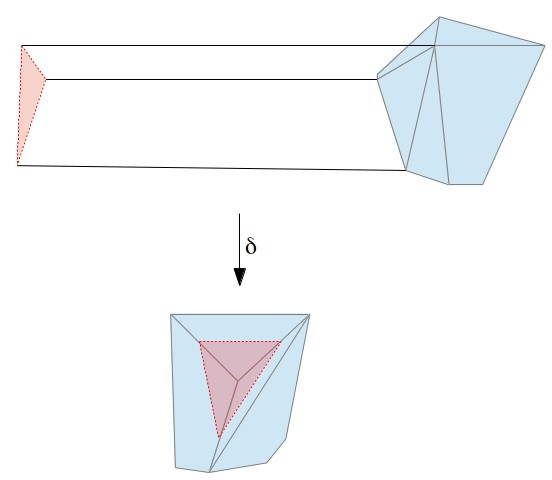
\includegraphics[width=10cm]{images/BlinkContourDual.jpg}
 \caption{Образ бликового контура при преобразовании двойственности.}
 \label{BlinkContourDual}
\end{figure}

Приведенный выше критерий можно проиллюстрировать с помощью рисунка
\ref{BlinkContourDual}. Заметим, что обозначенное на нижнем рисунке красным
цветом сечение не проходит ни через одну вершину двойственного многогранника.
Это связано с тем, что в противном случае одна из плоскостей граней исходного
многогранника обязана была бы быть плоскостью бликового цилиндра, что
невозможно.

В этом заключается принципиальное отличие бликовых и теневых контуров. Для
теневых контуров возможна такая их интерпретация, при которой
вершины двойственных образов теневых контуров являются вершинами двойственного
многогранника. Такая интерпретация возможна, если предположить, что каждый
теневой цилиндр составлен из плоскостей граней искомого многогранника.
Безусловно, такое предположение не реализуется в действительности, поскольку при
фотографировании одно и то же ребро появляется на нескольких кадрах сразу, и
почти наверное можно сказать, что ни на одном кадре нет скользящей проекции
ребра вдоль какой-нибудь инцидентной ему грани. Следуя
\cite{journals/pami/PrinceW90}, такую интерпретацию входных данных будем
называть \textbf{интерпретацией базового тела}.

\begin{figure}[ht]
 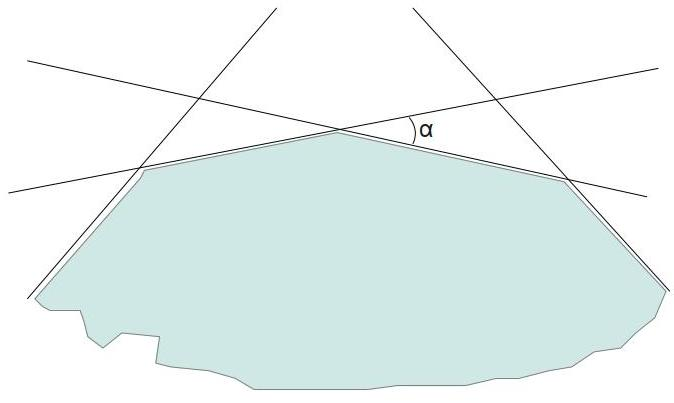
\includegraphics[width=10cm]{images/contour-1.jpg}
 \caption{Интерпретация базового тела}
 \label{contour-1}
\end{figure}

\begin{figure}[ht]
 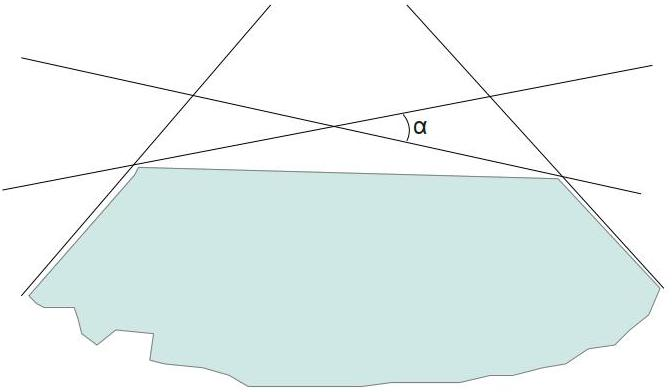
\includegraphics[width=10cm]{images/contour-2.jpg}
 \caption{Реальная конфигурация многогранника}
 \label{contour-2}
\end{figure}

Для наглядности на рисунках \ref{contour-1} и \ref{contour-2} показаны
интерпретация базового тела исходных входных данных и реальная конфигурация
многогранника, соответствующая таким входным данным.

Данная идея представляет из себя причину, по которой естественно возникает
потребность в разработке алгоритмов, учитывающих такую особенность входных
данных. Главная мотивация в этом деле -- снизить усложненность полученной
модели и попытаться приблизить ее к реальной конфигурации. Об этом будет
рассказано подробнее в последующих разделах.

Еще одно характерное отличие бликовых контуров от теневых -- это то, что они не
содержат начало координат в ограничиваемой ими конечной области плоскости. Это
существенным образом сказывается на свойствах образов этих контуров при
преобразовании двойственности. Для примера рассмотрим бликовый контур
$A_{1}A_{2}A_{3}A_{4}$, являющийся квадратом. изображенный на рисунке.
Введем на плоскости, в которой он лежит, двумерную систему координат $Oxy$.
Пусть вершины квадрата имеют координаты

\begin{align*}
& A_{1} = (1, 1), \\
& A_{2} = (3, 1), \\
& A_{3} = (3, -1), \\
& A_{4} = (1, -1) 
\end{align*}

тогда уравнения прямых, на которых лежат его стороны, представляют из себя
следующее:

\begin{align*}
& A_{1} A_{2}: \;\; y = 1 \\
& A_{2} A_{3}: \;\; \frac{1}{3} x = 1 \\
& A_{3} A_{4}: \;\; -y = 1 \\
& A_{4} A_{1}: \;\; x = 1
\end{align*}

При преобразовании двойственности вершины квадрата перейдут в следующие прямые:

\begin{align*}
& \delta(A_{1}) = \{ x + y = 1 \} \\
& \delta(A_{2}) = \{ 3 x + y = 1 \} \\
& \delta(A_{3}) = \{ 3 x - y = 1 \} \\
& \delta(A_{4}) = \{ x - y = 1 \}
\end{align*}

А прямые -- перейдут в следующие точки:

\begin{align*}
& \delta(A_{1} A_{2}) = (0, 1), \\
& \delta(A_{2} A_{3}) = (\frac{1}{3}, 0), \\
& \delta(A_{3} A_{4}) = (0, -1), \\
& \delta(A_{4} A_{1}) = (1, 0)
\end{align*}

Очевидно, что двойственный образ квадрата будет представлять из себя невыпуклый
четырехугольник (см. рис. \ref{BlinkSquareUnderDualTransform}).

\begin{figure}[ht]
 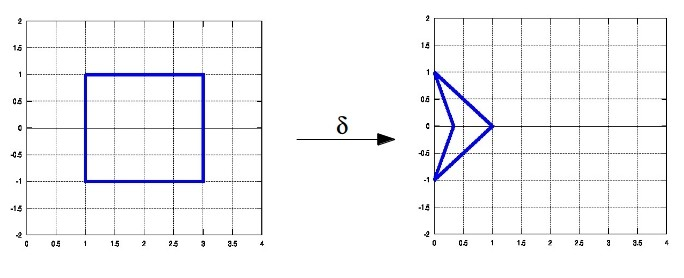
\includegraphics[width=10cm]{images/BlinkSquareUnderDualTransform.jpg}
 \caption{Бликовый контур, состоящий из квадрата и не содержащий начало
 координат, при преобразовании двойственности превращается в невыпуклый
 четырехугольник}
 \label{BlinkSquareUnderDualTransform}
\end{figure}



\subsection{Образы одной вершины на разных контурах}

Очевидно, что одна и та же вершина при фотографировании камня может иметь образы
на нескольких снимках сразу. Вне всякого сомнения, это определенным образом
должно отразиться на свойствах полученных контуров. Такая ситуация
характеризуется тем, что несколько (более одного) ребер последовательных теневых
цилиндров пересекаются в одной точке (см. рис. \ref{OneVertexOnMultiplePhotos}).
Существуют методы, которые позволяют находить с помощью кластеризации подобные
вершины, и по ним восстанавливать трехмерные модели.

\begin{figure}[ht]
 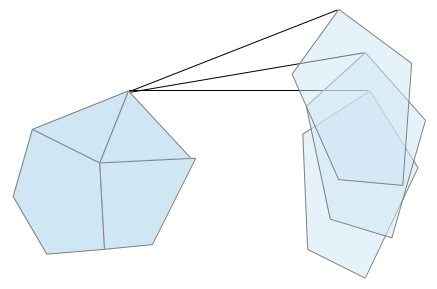
\includegraphics[width=10cm]{images/OneVertexOnMultiplePhotos.jpg}
 \caption{Образы одной вершины на разных контурах}
 \label{OneVertexOnMultiplePhotos}
\end{figure}

% TODO: Здесь нужно процитировать дипломную работу Степана. По всей видимости,
% он вводил определения и их здесь можно повторить...

В случае точных теневых контуров можно идентифицировать вершины разных контуров
как изображения одной и той же вершины исходного тела, если соответствующие
ребра теневых цилиндров пересекаются в одной точке. В реальном же случае,
когда все фотографии создаются с погрешностями, прямые могут и не пересечься.

Как можно идентифицировать изображения одной и той же вершины в двойственном
пространстве?

С точки зрения преобразования двойственности удобнее изучать этот вопрос в
терминах ребер. Пусть $e$ -- некоторое ребро исходного многогранника. Тогда для
тех кадров, на которых ребро $e$ видно, в соответствующих теневых цилиндрах
будет иметься по стороне, проходящей через $e$. Обозначим плоскости этих
сторон как $\pi_{1}, \pi_{2}, \ldots, \pi_{s}$. Все эти плоскости содержат в
себе (в реальном случае -- приближенно) ребро $e$:
$e \subset \pi_{i}, \;\; i = 1, 2, \ldots, s$. Поскольку преобразование
двойственности сохраняет отношение инцидентности между геометрическими
объектами, в двойственном пространстве полученные объекты будут снова
инцидентны друг другу. Образом ребра $e$ будет являться некоторый отрезок
$\delta(e)$, а образами плоскостей $\pi_{1}, \pi_{2}, \ldots, \pi_{s}$ --
точки $\delta(\pi_{1}), \delta(\pi_{2}), \ldots, \delta(\pi_{s}) \in e$,
содержащиеся во внутренности отрезка $e$.

Если же рассматривать некоторую вершину $v$, инцидентную ребрам
$e_{1}, \ldots, e_{k}$, то в двойственном пространстве она будет представлять
собой плоскость $\delta(v)$, содержащую в себе ребра
$\delta(e_{1}), \ldots, \delta(e_{k})$. Вершины-образы сторон теневых цилиндров
будут представлять собой точки, лежащие в одной плоскости, на сторонах одного
многоугольника.

Как изменятся выше приведенные суждения, если попытаться произвести их для
бликовых контуров? Всякая плоскость-сторона бликового цилиндра также проходит
через ребро $e$, изображением которого она является. Отличие от случая теневых 
контуров состоит в том, что стороны бликовых цилиндров не лежат между
плоскостями граней исходного многогранника, проходящих через это ребро. Для 
удобства можно ввести следующее определение:

\begin{SmartDefinition}
 Пусть $P$ -- многогранник в $\mathbb{R}^{3}$, $e$ -- некоторое ребро
многогранника $P$, а $f_{1}$ и $f_{2}$ -- содержащие его грани. Пусть $\pi_{1}$
и $\pi_{2}$ -- плоскости соответствующих граней. Тогда \textbf{углом теневой
видимости ребра} $e$ называется тот двугранный угол, образованный плоскостями
$\pi_{1}$ и $\pi_{2}$, который не содержит в себе внутренних точек
многогранника $P$ -- если такой двугранный угол существует.
\end{SmartDefinition}

В данных терминах можно сказать, что плоскости-стороны теневых цилиндров лежат
внутри углов теневой видимости соответствующих им ребер многогранника, а
плоскости-стороны бликовых цилиндров могут лежать, а могут и не лежать в этом
угле. В первом случае двойственные образы плоскостей-сторон будут являться
точками, лежащими на отрезке $e$, в последнем -- нет. Тем не менее, поскольку
$\alpha_{1}, \ldots, \alpha_{l}$ (бликовые плоскости-стороны) проходят через
обе точки $A_{1}$ и $A_{2}$ (вершины ребра $e$), их двойственные образы -- точки
$\delta(\alpha_{1}), \ldots, \delta(\alpha_{l})$ лежат в плоскостях
$\delta(A_{1})$ и $\delta(A_{2})$, то есть лежат на прямой, являющейся
пересечением этих плоскостей. Обозначим эту прямую через $l$. Верно утверждение,
что $\delta(\pi_{1}) \in l$ и $\delta(\pi_{2})$, где $\pi_{1}$ и $\pi_{2}$ --
стороны угла теневой видимости, т. е. плоскости граней многогранника $P$,
содержащие ребро $e$. Двойственные образы плоскостей-сторон теневых цилиндров
будут лежать на прямой $l$ между точками $\delta(\pi_{1})$ и $\delta(\pi_{2})$,
а плоскости-стороны бликовых цилиндров будут лежать на прямой $l$ вне отрезка
$\delta(e) = \delta(\pi_{1}) \delta(\pi_{2})$.

По какую сторону от отрезка $\delta(e)$ будет лежать двойственный образ той или 
иной бликовой плоскости-стороны? Рассмотрим такую бликовую плоскость-сторону 
$\pi_{0}$, которая помимо того, что проходит через отрезок $e$, содержит также 
в себе начало координат $O$ (т. е. рассмотрим плоскость $O A_{1} A_{2}$). 
Поскольку свободный член уравнения, описывающее плоскость $O A_{1} A_{2}$
равен $0$, то преобразование двойственности на нем не определено. Все бликовые 
плоскости-стороны, проходящие через ребро $e$, лежат либо по одну, либо по 
другую сторону от плоскости $O A_{1} A_{2}$. В зависимости от того, по какую 
сторону они лежат, точки, являющиеся их двойственными образами, будут лежать
по ту или по другую сторону от ребра $\delta(e)$ на прямой $l$ (см. рис.
\ref{DualShadowBlinkSides}).

\begin{figure}[ht]
 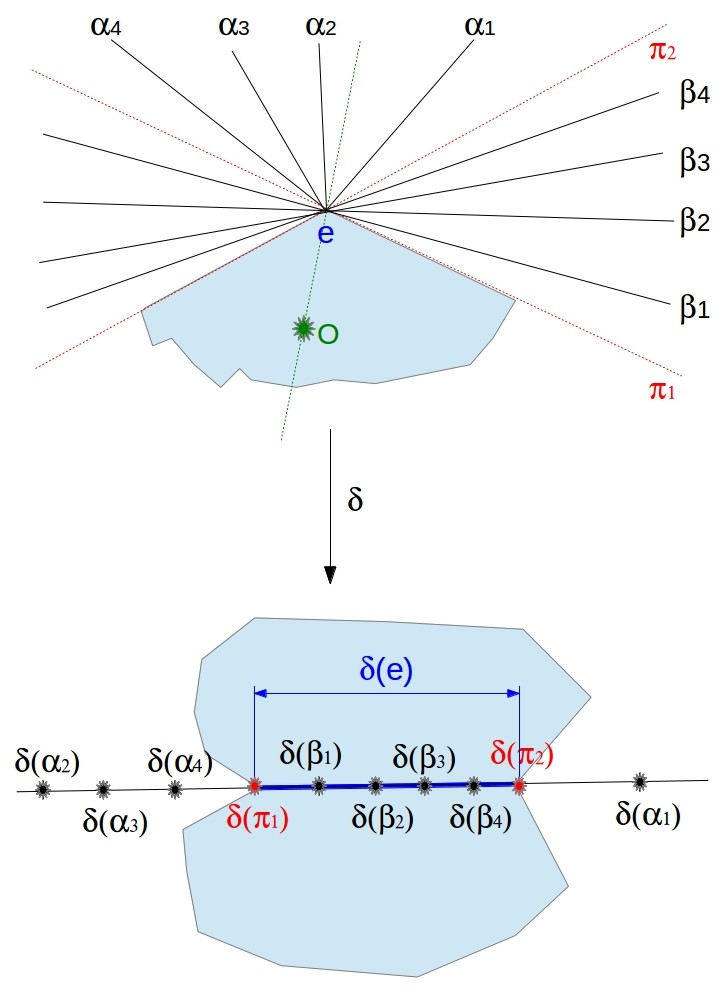
\includegraphics[width=10cm]{images/DualShadowBlinkSides.jpg}
 \caption{Двойственные образы плоскостей-сторон теневых и бликовых цилиндров}
 \label{DualShadowBlinkSides}
\end{figure}

\subsection{Разрешение нарушений плоскостности при подвижке вершины}

Отступим немного от принятой задачи восстановления и предположим, что уже
построено некоторое трехмерное тело. Допустим, что с целью устранения дефекта в
модели требуется подвинуть некоторую вершину из одного положения в другое.
Можно ли каким-то образом воспользоваться свойствами преобразования
двойственности, чтобы решить эту задачу?

Для простоты предположим, что построенный многогранник -- выпуклый. Для начала
рассмотрим задачу на простом примере. Пусть
$P = A_{0} A_{1} A_{2} A_{3} A_{4} A_{5} A_{6} A_{7}$ -- куб со
стороной длины $2$, координаты вершин которого имеют величины $-1$ и $1$. Его
вершины имеют следующие координаты:

\begin{align*}
 & A_{0} = (-1, -1, -1) \\ & A_{1} = (1, -1, -1) \\
 & A_{2} = (1, 1, -1)   \\ & A_{3} = (-1, 1, -1) \\
 & A_{4} = (-1, -1, 1)  \\ & A_{5} = (1, -1, 1)  \\
 & A_{6} = (1, 1, 1)    \\ & A_{7} = (-1, 1, 1)
\end{align*}

Уравнения плоскостей его граней имеют следующий вид:

\begin{align*}
 & A_{0} A_{1} A_{2} A_{3} : z = -1 \Leftrightarrow -z = 1 \\
 & A_{4} A_{5} A_{6} A_{7} : z = 1 \\
 & A_{0} A_{1} A_{5} A_{4} : y = -1 \Leftrightarrow -y = 1 \\
 & A_{1} A_{2} A_{6} A_{5} : x = 1 \\
 & A_{2} A_{3} A_{7} A_{6} : y = 1 \\
 & A_{3} A_{0} A_{4} A_{7} : x = -1 \Leftrightarrow -x = 1 \\
\end{align*}

% TODO: Добавить сюда изображение куба P.

Двойственные образы вершин куба представляют из себя плоскости, имеющие
следующие уравнения:

\begin{align*}
 & \delta(A_{0}) = \{ -x - y - z = 1 \} \\
 & \delta(A_{1}) = \{  x - y - z = 1 \} \\
 & \delta(A_{2}) = \{  x + y - z = 1 \} \\
 & \delta(A_{3}) = \{ -x + y - z = 1 \} \\
 & \delta(A_{4}) = \{ -x - y + z = 1 \} \\
 & \delta(A_{5}) = \{  x - y + z = 1 \} \\
 & \delta(A_{6}) = \{  x + y + z = 1 \} \\
 & \delta(A_{7}) = \{ -x + y + z = 1 \}
\end{align*}

Двойственные образы граней куба представляют из себя следующие точки:

\begin{align*}
 & \delta(A_{0} A_{1} A_{2} A_{3}) = ( 0,  0, -1) \\
 & \delta(A_{4} A_{5} A_{6} A_{7}) = ( 0,  0,  1) \\
 & \delta(A_{0} A_{1} A_{5} A_{4}) = ( 0, -1,  0) \\
 & \delta(A_{1} A_{2} A_{6} A_{5}) = ( 1,  0,  0) \\
 & \delta(A_{2} A_{3} A_{7} A_{6}) = ( 0,  1,  0) \\
 & \delta(A_{3} A_{0} A_{4} A_{7}) = (-1,  0,  0)
\end{align*}

Следовательно, двойственным образом куба $P$ является октаэдр $\delta(P)$ с
вершинами в концах единичных отрезков на осях координат $Ox$, $Oy$ и $Oz$.

% TODO: Добавить сюда изображение октаэдра \delta(P).

Пусть требуется подвинуть точку $A_{6} = (1, 1, 1)$ в некоторое новое положение
$A_{6}^{*} = (1 + d_{1}, 1 + d_{2}, 1 + d_{3})$.

\textbf{1. } Рассмотрим сначала случай $d_{1} > 0, d_{2}, d_{3} > 0$.

Если оставить все остальные вершины и грани куба без изменения, то трех гранях,
содержащих вершину $A_{6}$, т. е. в гранях
$A_{1} A_{2} A_{6} A_{5}, A_{2} A_{3} A_{7} A_{6}, A_{4} A_{5} A_{6} A_{7}$,
нарушится плоскостность, поскольку вершины этих граней теперь не будут лежать в
одной плоскости. Как эта ситуация выглядит в двойственном пространстве?

Очевидно, что всякое перемещение точки, удаляющее ее от начала координат,
соответствует перемещению ее двойственного образа, приближающему его к началу
координат в двойственном пространстве. В данном случае двойственный образ
вершины $A_{6}$ после перемещения будет представлять из себя следующее:

\begin{equation*}
 \delta(A_{6}^{*}) = \{ (1 + d_{1}) x + (1 + d_{2}) y + (1 + d_{3}) z = 1 \}
\end{equation*}

Новая плоскость по прежнему пересекает грани, смежные с ней по общему ребру, по
некоторому ребру, а грани, смежные с ней по вершине -- теперь пересекает по
некоторому новому образовавшемуся ребру (см. рис. ).

%%%%%%%%%%%%%%%%%%%%%%%%%%%%%%%%%%%%%%%%%%%%%%%%%%%%%%%%%%%%%%%%%%%%%%%%%%%%%%%%

\section{Опорные методы и опорные задачи восстановления выпуклых
тел (исторический обзор)}

В предыдущем разделе мы пытались рассматривать различные интерпретации входных
данных задачи восстановления трехмерного тела, назвали эти данные
\textit{задачами восстановления}. Однако строгого понятия \textit{решения
задачи восстановления} дано не было. В первую очередь это обусловлено самой
сущностью прикладной задачи, в которой строгого понимания, какой именно объект
в конечном счете нужно получить, -- нет. На практике требуется получить
тело, которое бы наилучшим образом приближало исходное (с точки зрения
близости в евклидовой метрике между вершинами, ребрами и гранями исходного и
восстановленного многогранников), -- с одной стороны, а с другой -- которое бы
повторяло основные топологические особенности тела.

Оказывается, существуют такие ситуации, когда эти две цели не могут быть
удовлетворены одновременно. На практике часто возникают ситуации, когда
построенная модель близко расположена к требуемым позициям в пространстве,
однако вместо одной крупной грани в ней присутствуют несколько более
мелких, или когда вместо одной вершины с большим числом инцидентных ей
ребер (т. е. высокой степени), однако в модели вместо одной вершины присутствуют
несколько близко расположенных вершин меньшей степени.

Любая математическая формализация задачи приводит к упрощению, если мы
формулируем задачи, которые можно эффективно решить с помощью существующих
вычислительных методов. Поэтому целесообразным выглядит подход, когда
предлагается \textit{несколько вариантов решения}, а пользователь программного
пакета имеет возможность выбирать среди них, а еще лучше -- "усреднять"
различные решения между собой, чтобы получить такое, которое бы
было бы удовлетворительно с точки зрения сразу нескольких критериев качества
модели.

В результате обзора некоторого количества статей из математических и
физических журналов по геометрической томографии, мат. статистике и компьютерной
геометрии было замечено сходство изучаемой задачи с теми, которые
рассматриваются в тех статьях. А именно, было замечено, что входные данные
задачи восстановления моделей алмазов можно переформулировать в терминах входных
данных некоторых задач геометрической томографии. Поскольку в этой смежной
области уже был накоплен заметный опыт решения подобных задач, мы попытались
перенять его, и чтобы это сделать, а также понять, насколько ценными будут
полученные алгоритмы, мы постарались ответить на следующие вопросы:

\begin{enumerate}
 \item Какие формализации задачи восстановления геометрических тел существуют в
геометрической томографии?
 \item Какие решения поставленных задач могут быть построены с помощью
разработанных методов?
 \item Каким образом можно интерпретировать нашу исходную задачу восстановления
тела по теневым (а также бликовым) контурам как задачу, которую можно решить с
помощью разработанных методов?
 \item Какую практическую ценность будут иметь полученные результаты?
 \item Можно ли модифицировать разработанные методы таким образом, чтобы
повысить ценность этих результатов?
\end{enumerate}

Если смотреть с точки зрения этого плана, то в предыдущем разделе мы несколько
забежали вперед, -- а именно, уже введен основной геометрический аппарат этих
статей, и на его основе произведено несколько попыток интерпретации исходной
задачи. В настоящем разделе мы постараемся осветить первые два пункта плана, а
в следующем -- приведем идею, позволяющую оптимизировать имеющиеся алгоритмы с
точки зрения быстродействия, а в еще одном разделе -- ответим на третий вопрос.

\subsection{Опорные задачи}

\subsection{Двухмерные опорные методы}

\subsection{Трехмерный метод восстановления базового тела}

\subsection{Трехмерный метод вершинного восстановления тела}

\subsection{Двухмерный метод обнаружения краев}

%%%%%%%%%%%%%%%%%%%%%%%%%%%%%%%%%%%%%%%%%%%%%%%%%%%%%%%%%%%%%%%%%%%%%%%%%%%%%%%%

\section{Эффективный критерий согласованности опорных данных}

\subsection{Критерий выпуклости многогранника}

\subsection{Связь между локальной согласованностью опорных данных и выпуклостью
многогранника в ребре}

\subsection{Критерий согласованности опорных данных}

%%%%%%%%%%%%%%%%%%%%%%%%%%%%%%%%%%%%%%%%%%%%%%%%%%%%%%%%%%%%%%%%%%%%%%%%%%%%%%%%

\section{Различные способы сведения исходной проблемы к опорным задачам}

\subsection{Наивная интерпретация сторон контуров как опорных плоскостей}

\subsection{Кластеризация вершин теневых контуров}

\subsection{Предварительная кластеризация и сведение к опорной задаче
вершинного восстановления}



%%%%%%%%%%%%%%%%%%%%%%%%%%%%%%%%%%%%%%%%%%%%%%%%%%%%%%%%%%%%%%%%%%%%%%%%%%%%%%%%

\section{Обобщение на невыпуклый случай}

\newpage
\bibliographystyle{plain}
\bibliography{references}

\end{document}
